Całość oprogramowania wykorzystuje język programowania \texttt{C++}. Projektowana oraz implementowana sieć składa się
z~dwóch typów modułów, stąd też pojawiła się potrzeba zainicjowania dwóch osobnych projektów -- jednego pod elementy
sieci LoRa oraz drugiego, dedykowanego dla modułu serwera sieciowego (ang. \textsl{webserver}), z~uwagi na zupełnie inną
platformę sprzętową. Firmware napisany został z~wykorzystaniem kilku różnych podejść:
\begin{itemize}[label=--]
    \item modułowego: każdy plik źródłowy odpowiada za zbiór funkcji wykonujących określone zadania (np. praca
          z~biblioteką do modułów LoRa zaimplementowana jest w~pliku \texttt{lora.cpp}),
    \item obiektowego: większość elementów kodu źródłowego jest reprezentowana w~postaci osobnego obiektu. Każdy
          z~nich posiada swoje funkcje oraz pełni określone zadania (np. obiekt \enquote{\texttt{bme}} ma za zadanie
          umożliwić współpracę z~sensorami dostępnymi na płytce czujników BME280, która podłączona jest do każdego
          modułu SLAVE).
\end{itemize}
Ponadto, z~uwagi na wykorzystanie modułów posiadających duże ilości pamięci RAM dostępnej na oprogramowanie,
wykorzystane zostały dostępne w~nowszych wersjach języka \texttt{C++} -- funkcje szablonowe (ang. \textsl{template
    functions}) lub pętle typu \texttt{for-range}. Są to elementy, które znacznie ułatwiły implementację kodu oraz
pozwoliły na minimalizację powtarzalności pewnych elementów.

\section{Framework oraz biblioteki\label{sect:framework-libraries}} Bazą do oprogramowania na wszystkich modułach jest
framework Arduino oraz jego modyfikacja pod platformę STM32 -- stm32duino, która pozwala na wykorzystanie pełnej
funkcjonalności rdzenia Arduino \cite{stm32duino-docs}. Pomimo tego, że biblioteki HAL (ang. \textsl{Hardware
    Abstraction Layer}) oraz framework STM32 są narzędziami dedykowanymi, w~przypadku tego projektu nie można było ich
zastosować. Oryginalna biblioteka do obsługi modułów rozszerzeń LoRa została wycofana z~użytku na rzecz nowszej
implementacji, pod nowszą wersję płytek Nucleo z~wbudowanym hardware.

\subsection{Wykorzystane biblioteki\label{sect:used-libs}} Do implementacji oprogramowania na wszystkie moduły
wykorzystanych zostało kilka bibliotek, które pozwalały na dodanie pełnego zakresu funkcjonalności do każdego
z~projektów.

W przypadku bibliotek zewnętrznych (niebędących częścią rdzenia Arduino) były to:
\begin{itemize}[label=--]
    \item STM32duino I-NUCLEO-LRWAN1: biblioteka do uruchomienia oraz pracy z~modułem rozszerzeń LoRa. Pozwala ona na
          pracę w~dwóch trybach: LoRaRadio -- implementacja wykorzystująca tylko standard dolnej warstwy sprzętowej LoRa
          oraz LoRaWAN -- dodająca możliwość podłączenia modułów do istniejącej sieci LoRa oraz wysyłanie i~odbieranie
          z~niej wiadomości,
    \item Adafruit BME280 Library: biblioteka dedykowana do modułów BME280, pozwalająca na zbieranie danych z~sensorów,
          wykorzystując do tego magistralę SPI albo I2C (w~zależności od posiadanego modułu rozszerzeń),
    \item Adafruit BusIO: uniwersalna biblioteka dodająca pewien poziom abstrakcji do komunikacji po magistralach I2C
          oraz SPI,
    \item WiFi101: biblioteka, która daje możliwość wykorzystania modułu WiFi obecnego na płytce Adafruit Feather M0
          (wykorzystanej do uruchomienia serwera w~sieci lokalnej).
\end{itemize}
Ponadto, wykorzystane zostały biblioteki I2C oraz SPI, dostępne w~rdzeniu Arduino. Potrzebne były one do uzyskania
komunikacji pomiędzy mikrokontrolerem Adafruit Feather M0 a~modułem WiFi, sensorami BM280 podłączonymi do modułów SLAVE
oraz do stworzenia połączenia pomiędzy modułem MASTER a~płytką z~serwerem sieci lokalnej.

\subsection{Ograniczenia związane z~wykorzystaniem Arduino oraz STM32duino\label{sect:framework-limits}} STM32duino,
pomimo tego, że ułatwił, bądź w~ogóle pozwolił na pracowanie z~wykorzystywanymi modułami, nie jest platformą idealną,
pozbawioną ograniczeń. Jedynym z~nich, które w~dość znacznym stopniu utrudniło implementację oprogramowania dla modułów
sieci, był brak przerwań programowych oraz ograniczone możliwości zastosowania przerwań sprzętowych. Stąd też pojawił
się wymóg zastosowania pewnych obejść, jednocześnie tracąc na wydajności implementowanego rozwiązania. Ponadto,
występowały też problemy związane z~działaniem magistrali I2C, tutaj w~przypadku modułów Feather oraz standardowego
Arduino -- niemożliwe było wykorzystanie wyświetlacza OLED pracującego na magistrali I2C oraz zarejestrowania samego
mikrokontrolera jako części, z~którą można komunikować się po tej magistrali.

\section{Implementacja oprogramowania elementów sieci\label{sect:firmware-network}} Zaprojektowana sieć składała się
w~sumie z~pięciu modułów -- 4~z~nich stanowiły elementy sieci LoRa, natomiast ostatni był wykorzystywany jako serwer
w~sieci lokalnej. W~projekcie nie została wykorzystana pełna funkcjonalność LoRaWAN oraz typowa dla niej architektura
(przedstawiona w~sekcji \ref{sect:lorawan}, rys. \ref{img:lorawan-architecture}), ponieważ implementacja takiego
rozwiązania jest bardzo kosztowna i~wymaga znacznie większej ilości elementów. Aby móc skorzystać ze specyfikacji
wymagane jest posiadanie bramy (ang. \textsl{gateway}) oraz serwerów odpowiedzialnych za przyłączanie urządzeń,
zarządzanie siecią oraz serwera aplikacyjnego. Z~uwagi na to zastosowana została dużo prostsza i~mniej wymagająca metoda
budowania sieci, opierająca się na wykorzystaniu modułów w~formie nadajników radiowych, pracujących w~standardzie LoRa.
Schemat ideowy budowanej sieci przedstawiony został na rys. \ref{img:network-schematic}.

\begin{figure}[!htbp]
    \centering
    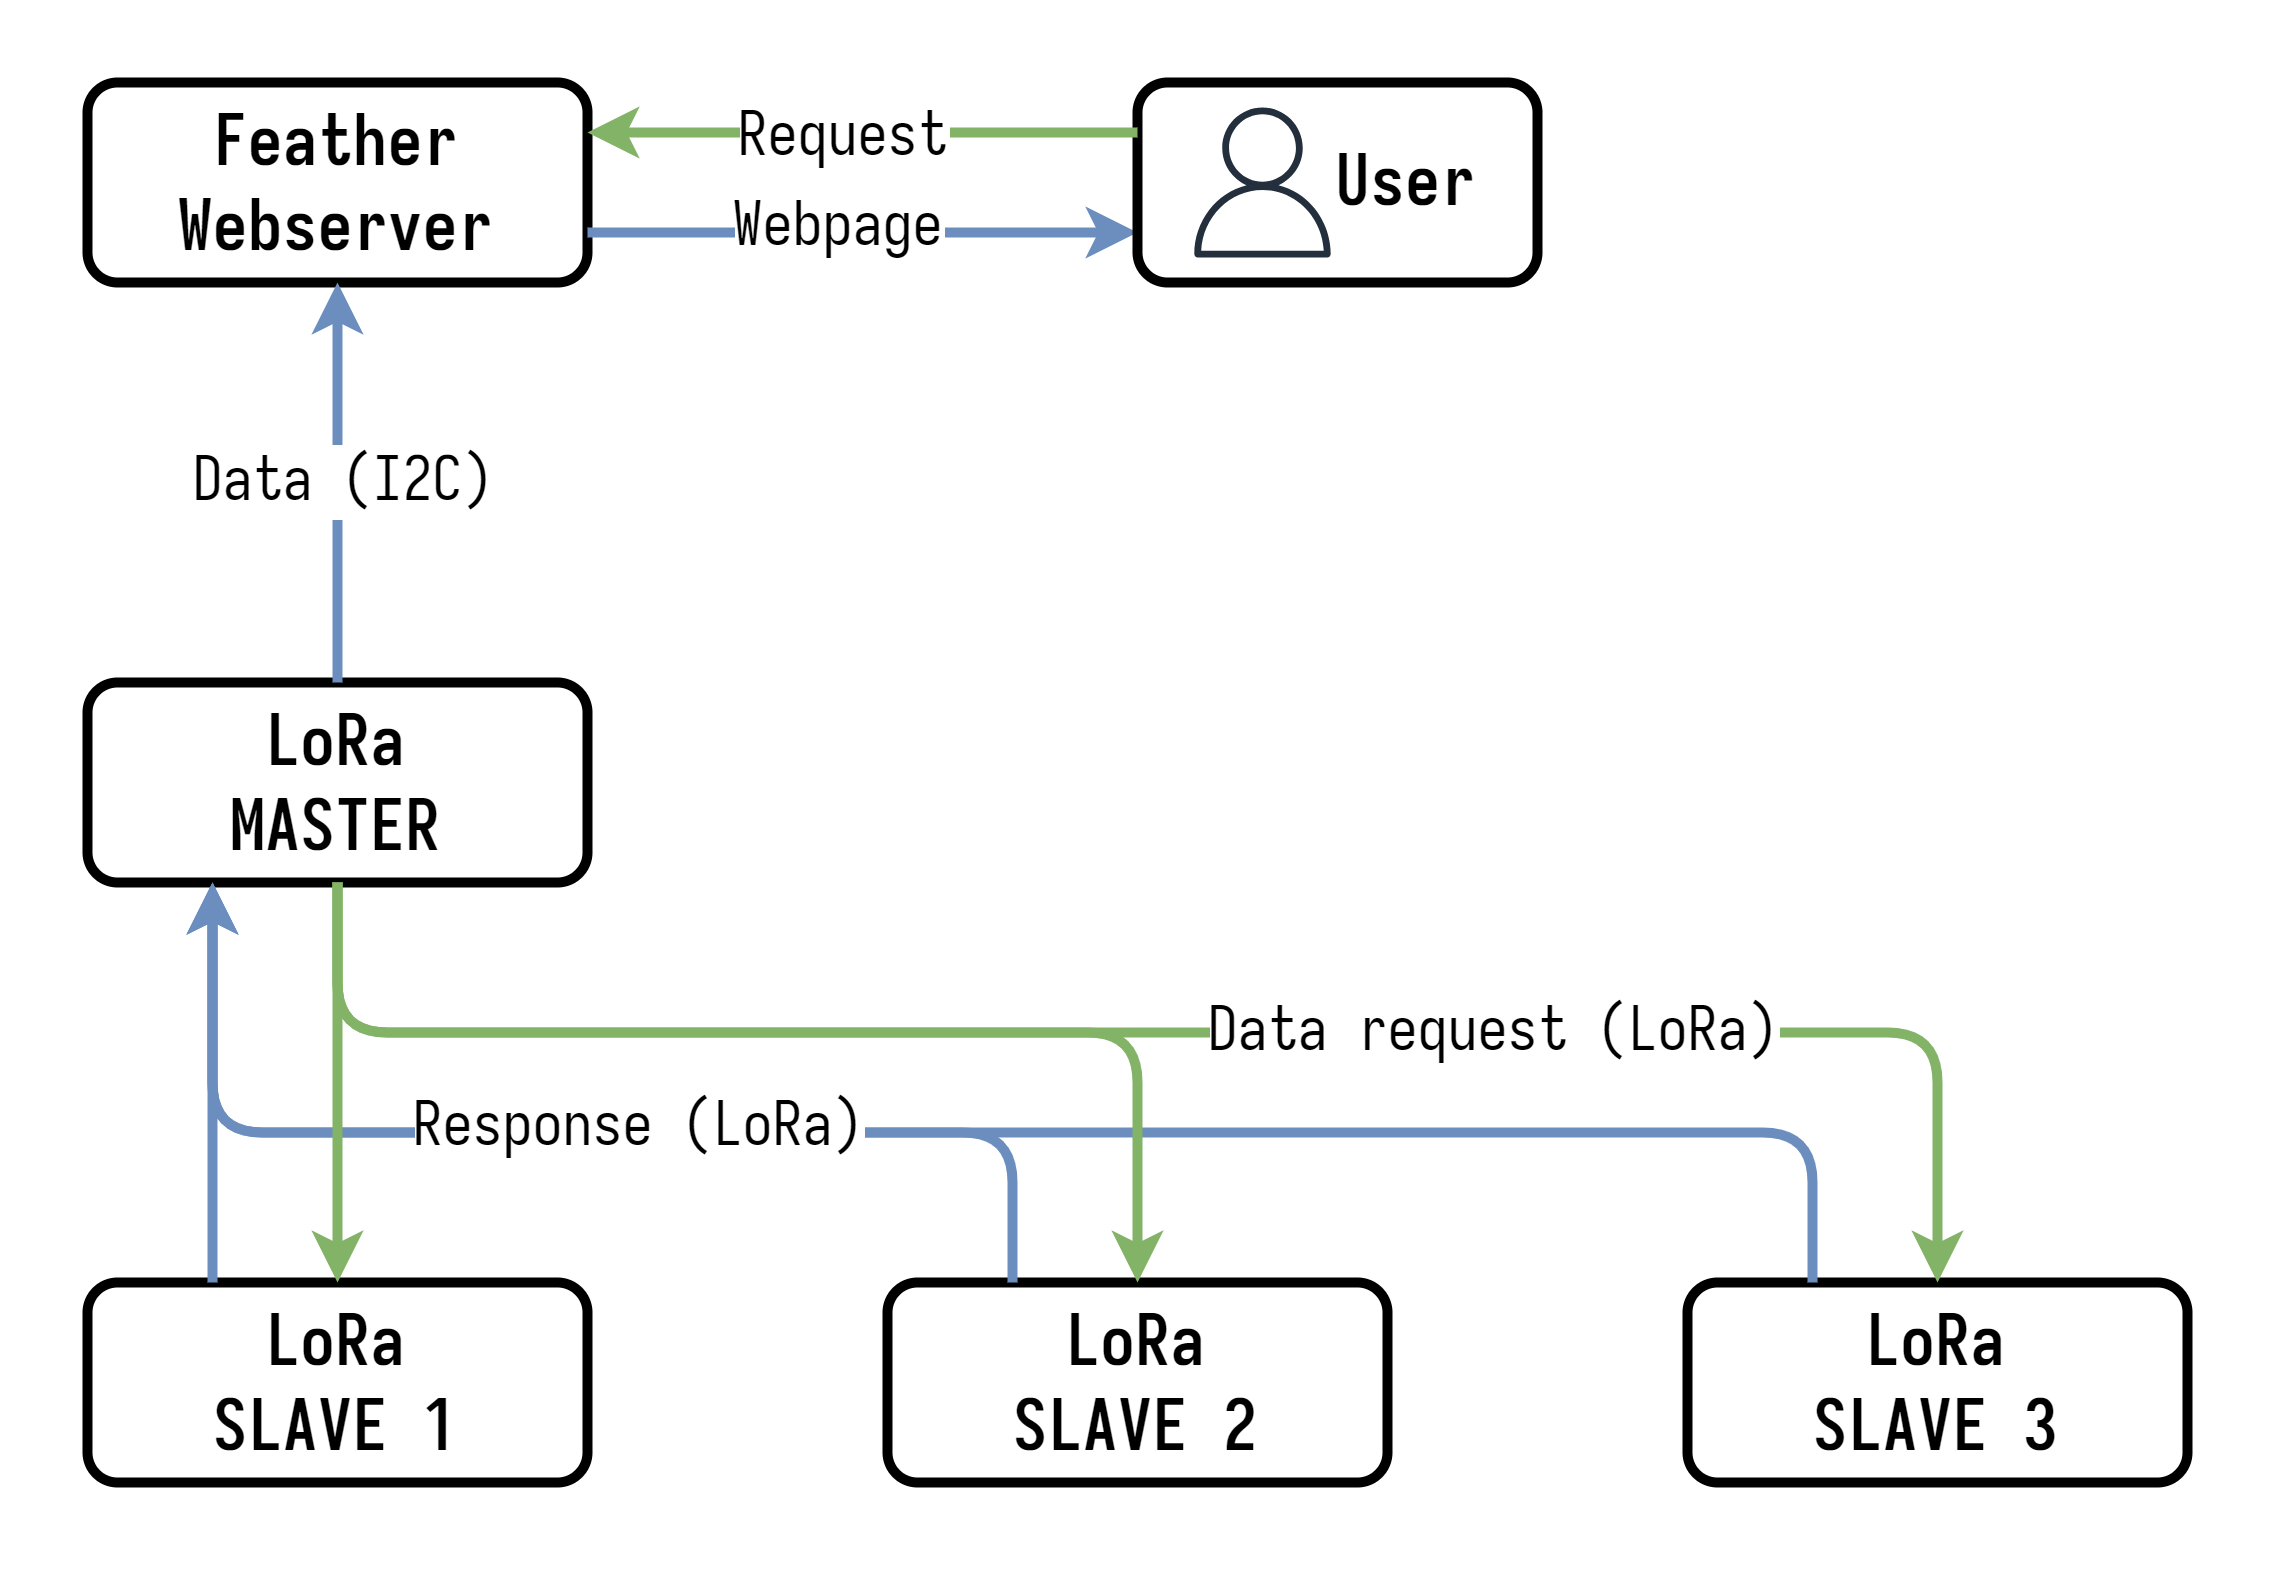
\includegraphics[width=0.7\textwidth]{schematics/network-schematic}
    \caption{\label{img:network-schematic}Schemat zbudowanej sieci, z~oznaczonymi elementami komunikacji}
\end{figure}

Oprogramowanie dla modułów pracujących w~sieci LoRa zostało zaimplementowane w~formie uniwersalnej -- jeden projekt
zawiera elementy dla modułu MASTER oraz modułów SLAVE. Plik konfiguracyjny projektu zawiera flagę, która definiuje, na
jaki typ modułu kod zostanie skompilowany. Co więcej, w~przypadku modułów SLAVE dodana została też flaga informująca
o~tym, jakie ID przypisane zostaje danej płytce. Rozwiązanie to odgrywa znaczącą rolę w~tym, jak wiadomości są
przesyłane w~sieci. Fragment pliku konfiguracyjnego, który odpowiedzialny jest za definiowanie tych elementów
przedstawiony został na listingu \ref{lst:lora-ini}.

\lstinputlisting[
    linerange={26-32},
    caption={Fragment pliku konfiguracyjnego (tutaj dla SLAVE1) odpowiedzialny za definicję typu oraz ID modułu},
    label={lst:lora-ini}
]{lora-psn/platformio.ini}

Wykorzystanie frameworku Arduino wymagało zastosowania pewnych schematów podczas implementacji. Dlatego też całość kodu
podzielona jest na dwie sekcje \texttt{setup()} oraz \texttt{loop()}, wykonywane odpowiednio raz, podczas startu modułu
oraz w~nieskończonej pętli, dopóki płytka ma zasilanie. Na rys. \ref{img:firmware-flowchart} przedstawiony został
schemat blokowy zaimplementowanego oprogramowania -- części zawartej w~sekcji \texttt{setup()}.

\begin{figure}[!htbp]
    \centering
    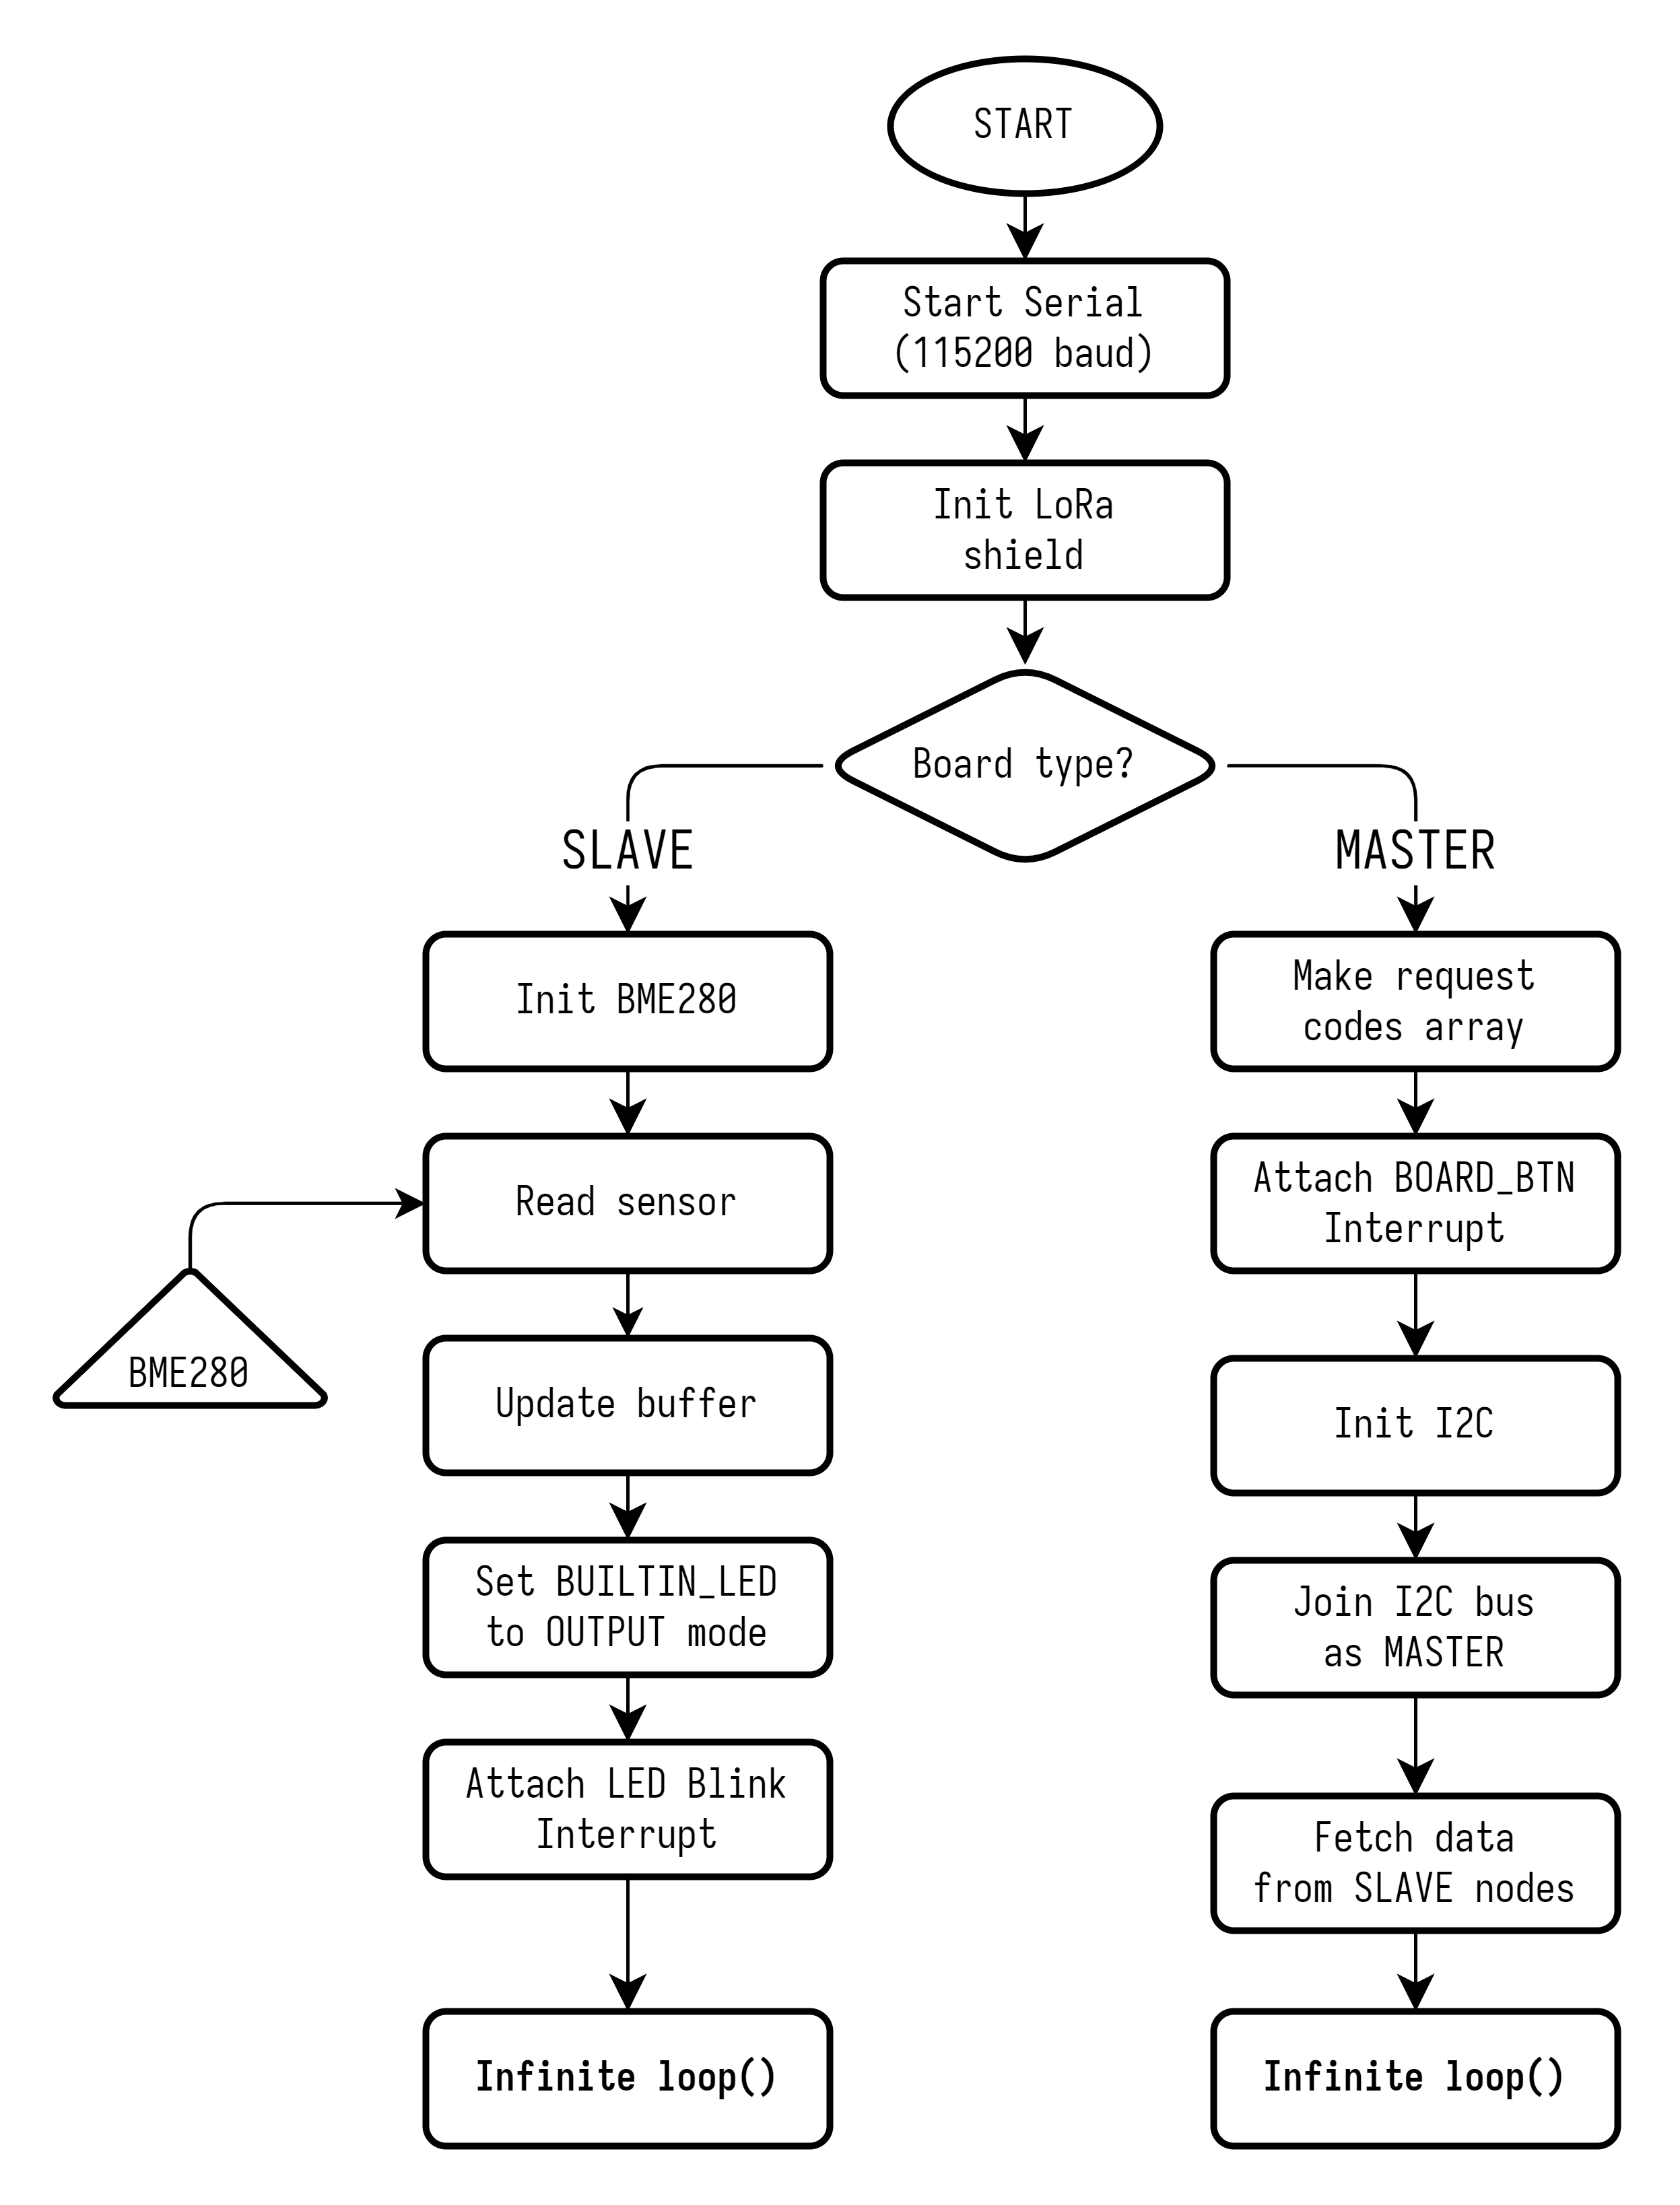
\includegraphics[width=0.9\textwidth]{firmware/firmware-flowchart}
    \caption{\label{img:firmware-flowchart}Schemat blokowy części \texttt{setup()} oprogramowania modułów sieci LoRa,
        z~podziałem na typ płytki}
\end{figure}

Oba typy oprogramowania zaczynają od ustawienia portu szeregowego na 115200 baud (szybkość transmisji), następnie
inicjowane jest rozszerzenie LoRa. Logowana jest informacja o~typie płytki, a~następnie kod oczekuje na informacje
o~starcie modułu rozszerzenia. W~przypadku błędu oraz poprawnego startu na port szeregowy wystawiana jest odpowiednia
informacja.

Następnie, w~zależności od typu płytki, wykonywane jest kilka operacji. W~przypadku modułów SLAVE są to:
\begin{enumerate}
    \item przygotowanie sensora BME280 oraz pobranie z~niego danych,
    \item aktualizacja zawartości bufora (wykorzystywanego do przechowywania odczytanych wartości),
    \item przygotowanie diody LED, która informuje o~trwającej komunikacji w~sieci,
    \item przygotowanie przerwania, wykorzystywanego do obsługi nowych zapytań.
\end{enumerate}

Natomiast dla modułów MASTER wykonywany jest inny zestaw operacji, z~uwagi na to, że taki moduł pełni zupełnie inną
funkcję w~sieci:
\begin{enumerate}
    \item przygotowanie tablicy z \enquote{kodami} zapytań (jedno bajtowe wartości do określenia czego żąda MASTER),
    \item inicjacja magistrali I2C i~podłączenie modułu jako MASTER,
    \item wykonanie podprogramu wysyłającego zapytania oraz odbierającego odpowiedzi od SLAVE-ów, tak aby tuż po
          starcie można było odczytać dane z~sieci.
\end{enumerate}
Ostatnim krokiem w~obu przypadkach jest przejście do nieskończonej pętli i~wykonywanie instrukcji w~niej zawartych,
wykorzystując do tego określony okres zegara.

\FloatBarrier
\subsection{Oprogramowanie modułu MASTER\label{sect:firmware-master}}

\subsection{Oprogramowanie modułów SLAVE\label{sect:firmware-slave}}

\section{Implementacja oprogramowania modułu serwera sieciowego\label{sect:firmware-webserver}}